\documentclass[parskip=full,11pt]{scrartcl}
\usepackage[utf8]{inputenc}

\title{\Huge Parkview\\
    \LARGE \normalfont Performance Dashboard for Continuous Benchmarking of HPC Libraries}
\author{Chingun Ariunbat, Jamil Bagga, Walter Alexander B\"ottcher,\\Darius Schefer, Maximilian Schik}

% section numbers in margins:
\renewcommand\sectionlinesformat[4]{\makebox[0pt][r]{#3}#4}

% header & footer
\usepackage{scrlayer-scrpage}
%\lofoot{\today} % Date in footer
\refoot{\today}  % no idea what this does
\pagestyle{scrheadings}

\usepackage[sfdefault,light]{roboto}
\usepackage[T1]{fontenc}
\usepackage[english]{babel}
\usepackage[yyyymmdd]{datetime} % must be after babel
\usepackage{float}
\renewcommand{\dateseparator}{-}
\usepackage[colorlinks=true, linkcolor=blue]{hyperref}
\usepackage{amsmath} % for $\text{}$
\usepackage[nameinlink]{cleveref}
\crefname{figure}{Abb}{Abb}
\usepackage[section]{placeins}
\usepackage{xcolor}
\usepackage[nonumberlist, toc]{glossaries}     % provides glossary commands, [toc] to appear in table of contents
\usepackage{graphicx}
\usepackage{dirtree}
\graphicspath{ {./images/} }
\hypersetup{
	pdftitle={Design},
	bookmarks=true
}
\usepackage{design}
\usepackage{csquotes} % provides \enquote{} command

\makenoidxglossaries

\newglossaryentry{developer}
{
	name=developer,
	plural=developers,
	description={Person working on the project that is to be benchmarked}
}

\newglossaryentry{configuration}
{
	name=configuration,
	plural=configurations,
	description={A complete description of a \gls{visualization}. It contains all the necessary information except the benchmark data.}
}

\newglossaryentry{template}
{
	name=template,
	plural=templates,
	description={A partial configuration of a \gls{visualization}. It contains preconfigured values, but leaves others blank for the user to costumize.}
}

\newglossaryentry{visualization}
{
	name=visualization,
	plural=visualizations,
	description={A graphical representation of benchmark data.}
}

\newacronym{ci}{CI}{Continuous Integration}

\newacronym{json}{JSON}{JavaScript Object Notation}
 % glossary header

\begin{document}

\maketitle
\begin{figure}[h]
	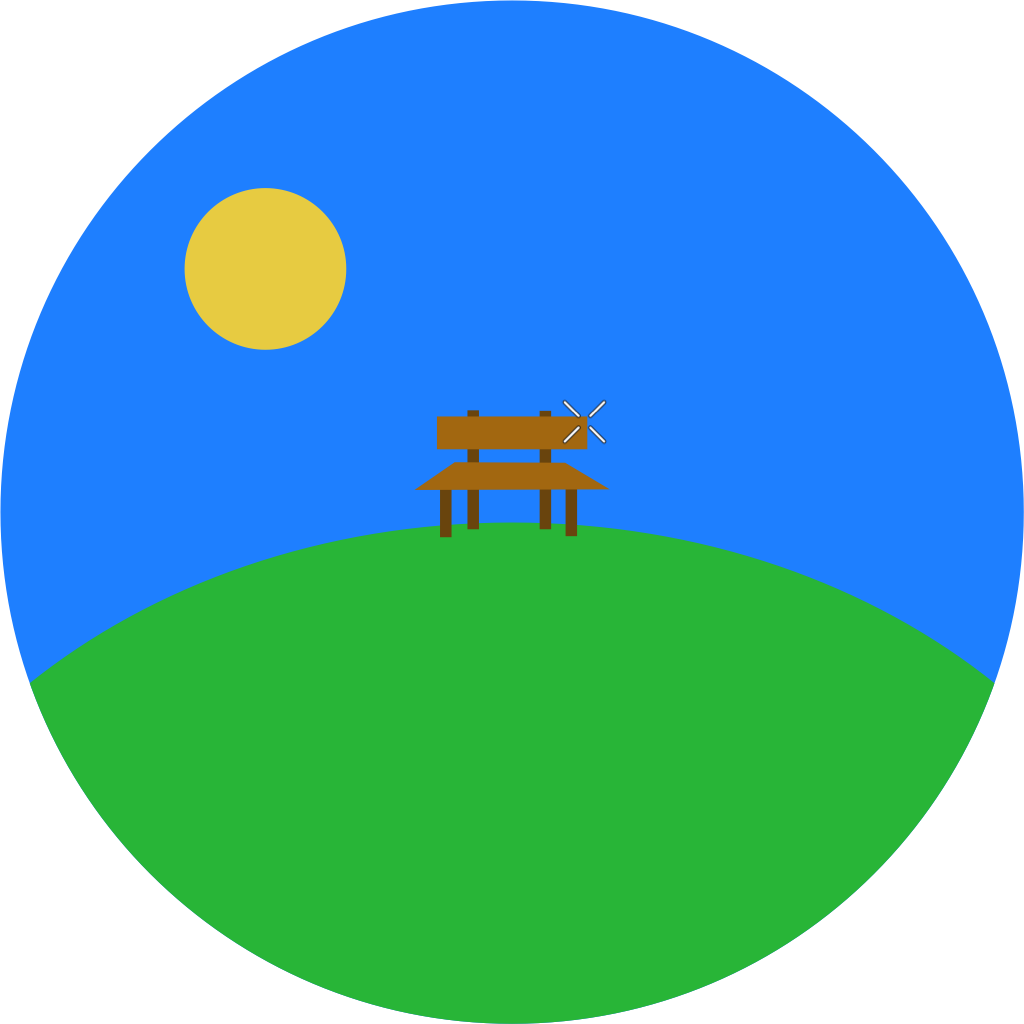
\includegraphics[width=11cm]{parkview.png}
	\centering
\end{figure}

\thispagestyle{empty}

\clearpage
\pagenumbering{arabic}

\tableofcontents
\clearpage

\section{Introduction}
This \gls{document} describes in detail the architecture of \parkview{}. The overall structure of the front- and backend is laid out using class diagrams and a more detailed view into the different functionalities is provided with sequence diagrams.
\clearpage

\section{Structure}
\begin{figure}[h]
	\centering
	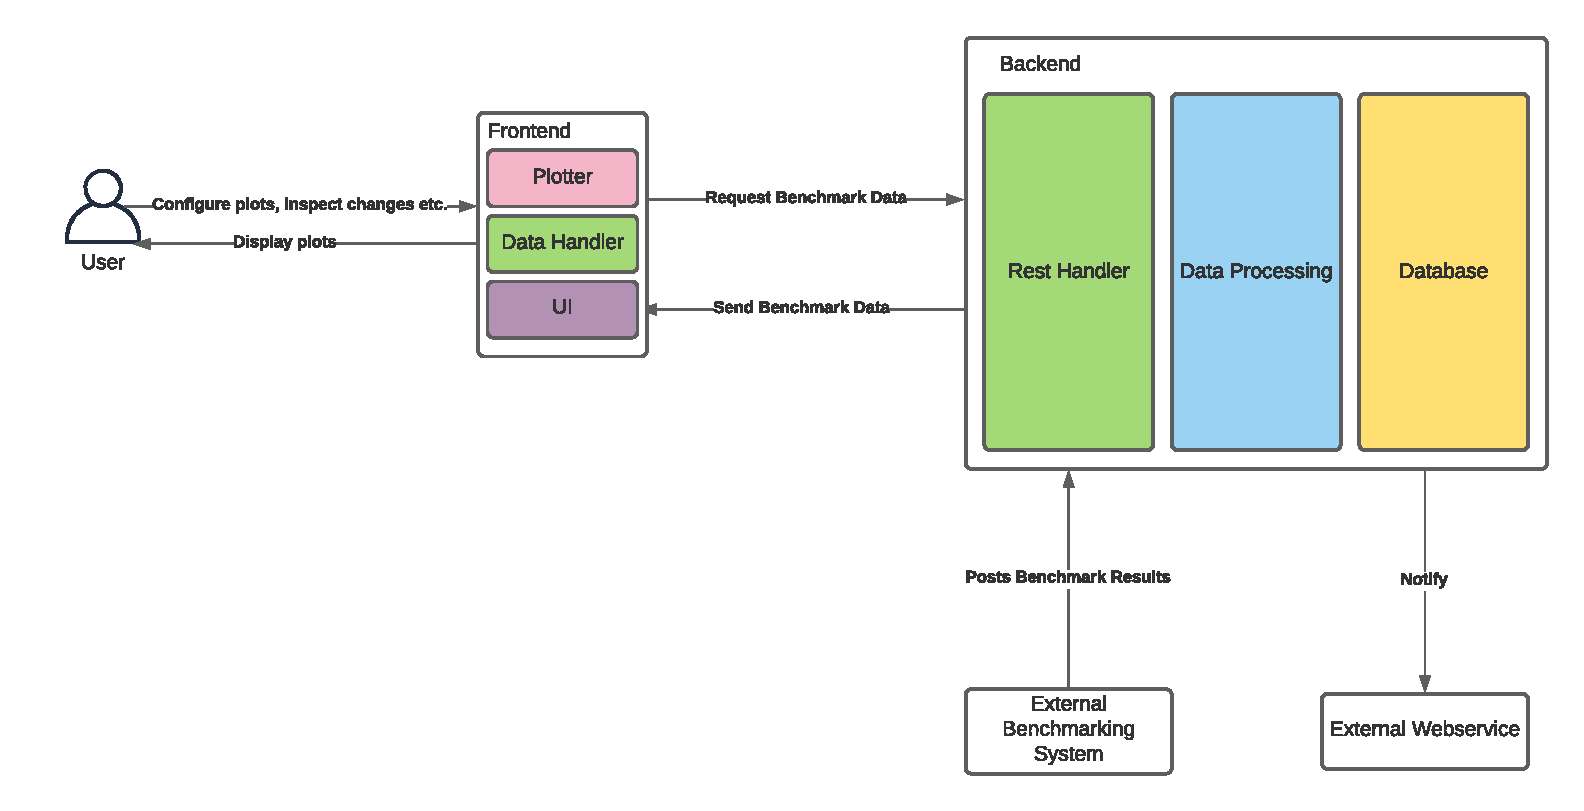
\includegraphics[width=\textwidth]{systemmodel.pdf}
	\caption{System Model}
\end{figure}

\subsection{Frontend}
The frontend is the primary interface the user interacts with and is responsible for displaying data.
\begin{figure}[h]
	\centering
	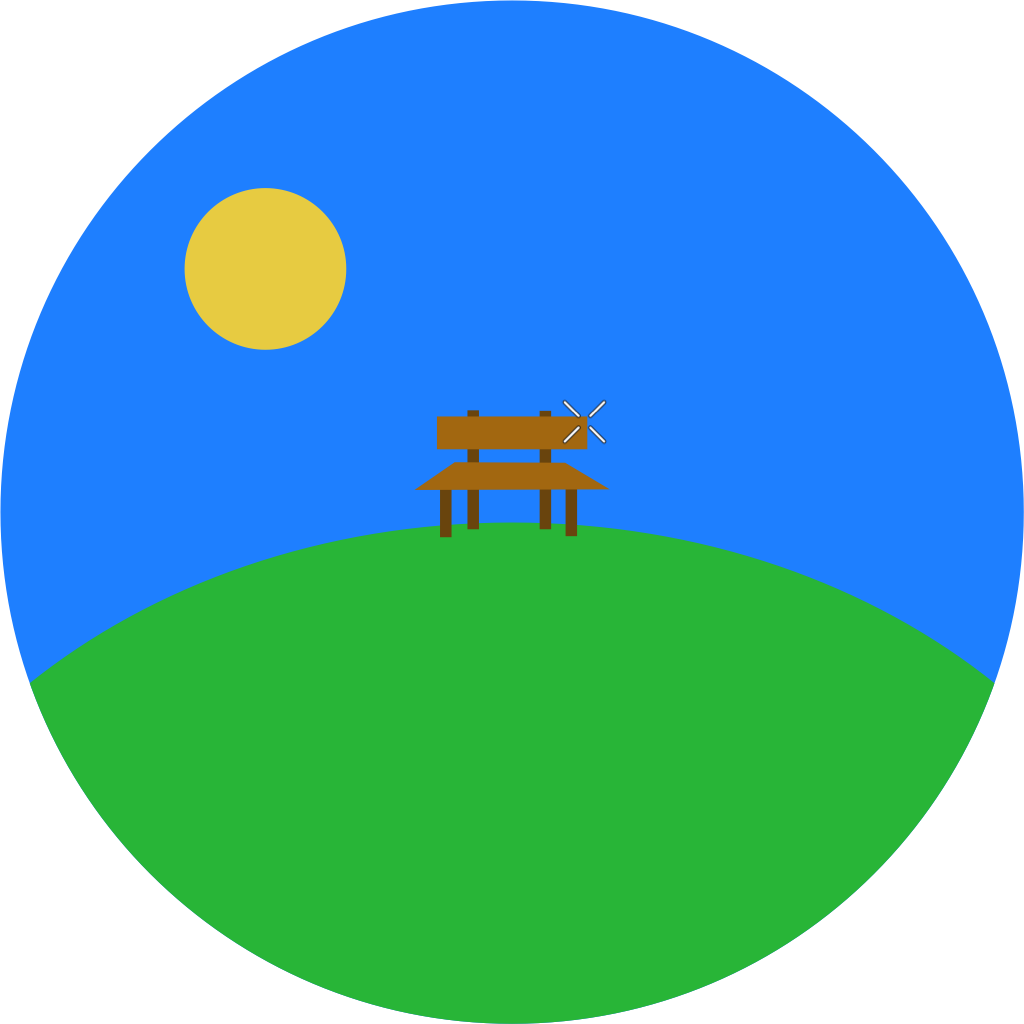
\includegraphics[scale=0.1]{parkview.png}
	\caption{Insert frontend class diagram here}
\end{figure}

\subsection{Backend}
The backend is responsible for handling the benchmark data and communicating with external actors such as webservices
\begin{figure}[h]
	\centering
	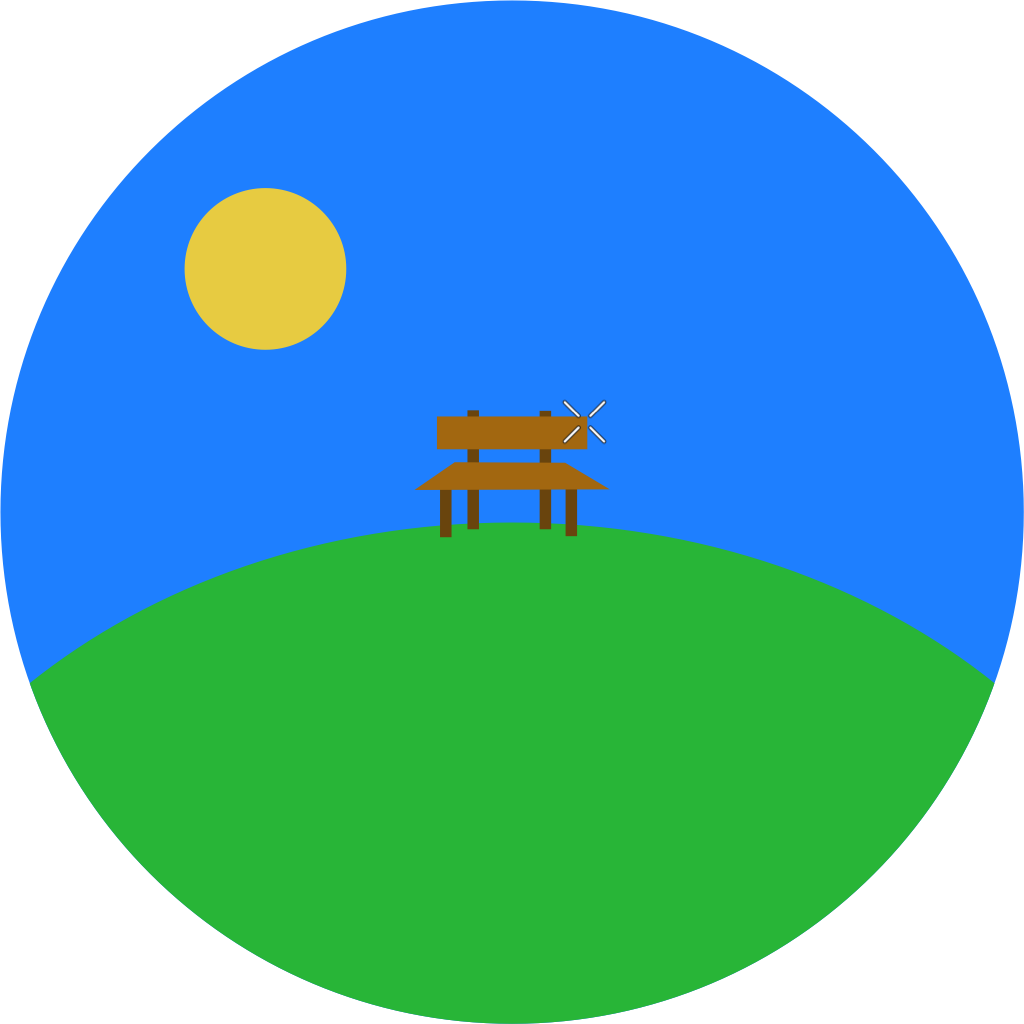
\includegraphics[scale=0.1]{parkview.png}
	\caption{Insert backend class diagram here}
\end{figure}

\clearpage

\section{Class descriptions}

Class descriptions here


\subsection{Frontend}
Frontend classes here

\class{Example Class : Parent Class}
{An example class, \\ very cool}
{
  \begin{itemize}
    \item \identifier{public int attr}{an attribute}
    \item \identifier{private int attr2}{another attribute}
    \item \identifier{private int attr3}{yet another attribute}
  \end{itemize}
}
{
  \begin{itemize}
    \item \identifier{public String getName()}{a method}
    \item \identifier{public int getNum()}{yet another method}
    \item \identifier{public void setNum(int num)}{guess what, a method}
  \end{itemize}
}

\subsection{Backend}
\subsubsection{benchmark}
\interface{BenchmarkResultStorage}
{This interface provides methods for the storage of benchmark results.}
{
  \begin{itemize}
      \item \identifier{void storeBenchmarkResults(results: List<BenchmarkResult>)}{Stores the given benchmark results in the database. If the benchmark result already exists, it gets replaced.}
  \end{itemize}
}

\class{BlasBenchmarkResult : BenchmarkResult}
{This is a benchmark result for the benchmarks of the BLAS format and type.}
{
  \begin{itemize}
    \item \identifier{private List<BlasDatapoint> datapoints}{List of datapoints belonging to this benchmark run.}
  \end{itemize}
}
{
  \begin{itemize}
      \item \identifier{public List<BlasDatapoint> getDatapoints()}{Getter for \texttt{datapoints}.}
  \end{itemize}
}

\class{BlasDatapoint}
{A single datapoint for the \texttt{BlasBenchmarkResult}, contains the problem description (n, r, m, k) and a list of operations.}
{
  \begin{itemize}
      \item \identifier{private int n}{n-value for this benchmark run.}
      \item \identifier{private int r}{r-value for this benchmark run.}
      \item \identifier{private int m}{m-value for this benchmark run.}
      \item \identifier{private int k}{k-value for this benchmark run.}
      \item \identifier{private List<Operation> operations}{List of operations, part of the benchmark.}
  \end{itemize}
}
{
  \begin{itemize}
      \item \identifier{public int getN()}{Getter for \texttt{n}.}
      \item \identifier{public int getR()}{Getter for \texttt{r}.}
      \item \identifier{public int getM()}{Getter for \texttt{m}.}
      \item \identifier{public int getK()}{Getter for \texttt{k}.}
      \item \identifier{public List<Operation> getOperations()}{Getter for \texttt{operations}.}
  \end{itemize}
}

\class{Component}
{A single component, part of \texttt{PreconditionerBenchmarkResult} and \texttt{SolverBenchmarkResult}.}
{
  \begin{itemize}
      \item \identifier{private String name}{Name of component.}
      \item \identifier{private double runtime}{Runtime for component.}
  \end{itemize}
}
{
  \begin{itemize}
      \item \identifier{public String getName()}{Getter for \texttt{name}.}
      \item \identifier{public double getRuntime()}{Getter for \texttt{runtime}.}
  \end{itemize}
}

\class{Conversion}
{A single conversion, part of \texttt{ConversionBenchmarkResult}.}
{
  \begin{itemize}
      \item \identifier{private String name}{Name of component.}
      \item \identifier{private double time}{Time to conversion.}
      \item \identifier{private bool completed}{Whether or not the benchmark has completed.}
  \end{itemize}
}
{
  \begin{itemize}
      \item \identifier{public String getName()}{Getter for \texttt{name}.}
      \item \identifier{public double getTime()}{Getter for \texttt{time}.}
      \item \identifier{public bool isCompleted()}{Getter for \texttt{completed}.}
  \end{itemize}
}

\class{ConversionBenchmarkResult : MatrixBenchmarkResult}
{This is a benchmark result for the benchmarks of the Conversion format and type.}
{ \\ }
{ \\ }

\class{ConversionDatapoint : MatrixDatapoint}
{A single datapoint for \texttt{ConversionBenchmarkResult}, contains the problem description for the matrix and a list of conversions.}
{
  \begin{itemize}
      \item \identifier{private List<Conversion> conversions}{List of conversions belonging to this benchmark run.}
  \end{itemize}
}
{
  \begin{itemize}
      \item \identifier{public int getConversions()}{Getter for \texttt{conversions}.}
  \end{itemize}
}

\class{Format}
{A single format, part of \texttt{SpmvBenchmarkResult}.}
{
  \begin{itemize}
      \item \identifier{private String name}{Name of format.}
      \item \identifier{private int storage}{}
      \item \identifier{private double time}{Time to format.}
      \item \identifier{private double maxRelativeNorm2}{}
      \item \identifier{private bool completed}{Whether or not this format has completed.}
  \end{itemize}
}
{
  \begin{itemize}
      \item \identifier{public String getName()}{Getter for \texttt{name}.}
      \item \identifier{public int getStorage()}{Getter for \texttt{storage}.}
      \item \identifier{public double getTime()}{Getter for \texttt{time}.}
      \item \identifier{public double getMaxRelativeNorm2()}{Getter for \texttt{maxRelativeNorm2}.}
      \item \identifier{public bool isCompleted()}{Getter for \texttt{completed}.}
  \end{itemize}
}

\class{MatrixBenchmarkResult : BenchmarkResult}
{Benchmark type that uses matrices.}
{
  \begin{itemize}
      \item \identifier{private List<MatrixDatapoint> datapoints}{List of datapoints belonging to this benchmark run.}
  \end{itemize}
}
{
  \begin{itemize}
      \item \identifier{public List<MatrixDatapoint> getDatapoints()}{Getter for \texttt{datapoints}.}
  \end{itemize}
}

\class{MatrixDatapoint}
{Single datapoint for a \texttt{MatrixBenchmarkResult}. Contains problem description (rows, columns, nonzeros).}
{
  \begin{itemize}
      \item \identifier{private String filename}{Filename for this benchmark run.}
      \item \identifier{private int rows}{Number of rows.}
      \item \identifier{private int columns}{Number of columns.}
      \item \identifier{private int nonzeros}{Number of non-zeros.}
  \end{itemize}
}
{
  \begin{itemize}
      \item \identifier{public String getFilename()}{Getter for \texttt{filename}.}
      \item \identifier{public int getRows()}{Getter for \texttt{rows}.}
      \item \identifier{public int getColumns()}{Getter for \texttt{columns}.}
      \item \identifier{public int getNonzeros()}{Getter for \texttt{nonzeros}.}
  \end{itemize}
}

\class{Operation}
{A single operation, part of \texttt{BlasBenchmarkResult}.}
{
  \begin{itemize}
      \item \identifier{private String name}{Name of operation.}
      \item \identifier{private double time}{}
      \item \identifier{private double flops}{}
      \item \identifier{private double bandwidth}{}
      \item \identifier{private bool completed}{Whether or not this operation has completed.}
  \end{itemize}
}
{
  \begin{itemize}
      \item \identifier{public String getName()}{Getter of \texttt{name}.}
      \item \identifier{public double getTime()}{Getter of \texttt{time}.}
      \item \identifier{public double getFlops()}{Getter of \texttt{flops}.}
      \item \identifier{public double getBandwidth()}{Getter of \texttt{bandwidth}.}
      \item \identifier{public bool getCompleted()}{Getter of \texttt{completed}.}
  \end{itemize}
}

\class{Preconditioner}
{A single preconditioner, part of \texttt{PreconditionerBenchmarkResult}.}
{
  \begin{itemize}
      \item \identifier{private String name}{Name of preconditioner.}
      \item \identifier{private List<Component> generateComponents}{}
      \item \identifier{private double generateTime}{}
      \item \identifier{private List<Component> applyComponents}{}
      \item \identifier{private double applyTime}{}
      \item \identifier{private bool completed}{Whether or not this preconditioner has completed.}
  \end{itemize}
}
{
  \begin{itemize}
      \item \identifier{private String getName()}{Getter for \texttt{name}.}
      \item \identifier{private List<Component> getGenerateComponents()}{Getter for \texttt{generateComponents}.}
      \item \identifier{private double getGenerateTime()}{Getter for \texttt{generateTime}.}
      \item \identifier{private List<Component> getApplyComponents()}{Getter for \texttt{applyComponents}.}
      \item \identifier{private double getApplyTime()}{Getter for \texttt{applyTime}.}
      \item \identifier{private bool isCompleted()}{Getter for \texttt{completed}.}
  \end{itemize}
}

\class{PreconditionerBenchmarkResult : MatrixBenchmarkResult}
{This is a benchmark result for the benchmarks of the Preconditioner format and type.}
{ \\ }
{ \\ }

\class{PreconditionerDatapoint : MatrixDatapoint}
{A single datapoint for \texttt{PreconditionerBenchmarkResult}, contains the problem description for the matrix and a list of preconditioners.}
{
  \begin{itemize}
      \item \identifier{private List<Preconditioner> preconditioners}{List of preconditioners belonging to this benchmark run.}
  \end{itemize}
}
{
  \begin{itemize}
      \item \identifier{public List<Preconditioner> getPreconditioners()}{Getter for \texttt{preconditioners}.}
  \end{itemize}
}

\class{Solver}
{A single Solver, part of \texttt{SolverBenchmarkResult}.}
{
  \begin{itemize}
      \item \identifier{private String name}{Name of solver.}
      \item \identifier{private List<double> recurrentResiduals}{}
      \item \identifier{private List<double> trueResiduals}{}
      \item \identifier{private List<double> implicitResiduals}{}
      \item \identifier{private List<double> iterationTimestamps}{}
      \item \identifier{private List<double> rhsNorm}{}
      \item \identifier{private List<double> residualNorm}{}
      \item \identifier{private List<Component> generateComponents}{}
      \item \identifier{private double generateTime}{}
      \item \identifier{private List<Component> applyComponents}{}
      \item \identifier{private double applyTime}{}
      \item \identifier{private int applyIterations}{}
      \item \identifier{private bool completed}{Whether or not this solver has completed.}
  \end{itemize}
}
{
  \begin{itemize}
      \item \identifier{public String getName()}{Getter for \texttt{name}.}
      \item \identifier{public List<double> getRecurrentResiduals()}{Getter for \texttt{recurrentResiduals}.}
      \item \identifier{public List<double> getTrueResiduals()}{Getter for \texttt{trueResiduals}.}
      \item \identifier{public List<double> getImplicitResiduals()}{Getter for \texttt{implicitResiduals}.}
      \item \identifier{public List<double> getIterationTimestamps()}{Getter for \texttt{iterationTimestamps}.}
      \item \identifier{public List<double> getRhsNorm()}{Getter for \texttt{rhsNorm}.}
      \item \identifier{public List<double> getResidualNorm()}{Getter for \texttt{residualNorm}.}
      \item \identifier{public List<Component> getGenerateComponents()}{Getter for \texttt{generateComponents}.}
      \item \identifier{public double getGenerateTime()}{Getter for \texttt{generateTime}.}
      \item \identifier{public List<Component> getApplyComponents()}{Getter for \texttt{applyComponents}.}
      \item \identifier{public double getApplyTime()}{Getter for \texttt{applyTime}.}
      \item \identifier{public int getApplyIterations()}{Getter for \texttt{applyIterations}.}
      \item \identifier{public bool getCompleted()}{Getter for \texttt{completed}.}
  \end{itemize}
}

\class{SolverBenchmarkResult : MatrixBenchmarkResult}
{This is a benchmark result for the benchmarks of the Solver format and type.}
{ \\ }
{ \\ }

\class{SolverDatapoint : MatrixDatapoint}
{A single datapoint for \texttt{SolverBenchmarkResult}, contains the problem description for the matrix and a list of solvers.}
{
  \begin{itemize}
      \item \identifier{private List<Solver> solvers}{List of solvers belonging to this benchmark run.}
  \end{itemize}
}
{
  \begin{itemize}
      \item \identifier{public int getSolvers()}{Getter for \texttt{solvers}.}
  \end{itemize}
}

\class{SpmvBenchmarkResult : MatrixBenchmarkResult}
{This is a benchmark result for the benchmarks of the SPMV format and type.}
{ \\ }
{ \\ }

\class{SpmvDatapoint : MatrixDatapoint}
{A single datapoint, contains the problem description for the matrix and a list of formats.}
{
  \begin{itemize}
      \item \identifier{private List<Format> formats}{List of formats belonging to this benchmark run.}
      \item \identifier{private Format optimal}{Optimal format for this benchmark run.}
  \end{itemize}
}
{
  \begin{itemize}
      \item \identifier{public List<Format> getFormats()}{Getter for \texttt{formats}.}
      \item \identifier{public Format getOptimal()}{Getter for \texttt{optimal}.}
  \end{itemize}
}

\subsubsection{database}

\class{BenchmarkResultDatabase : BenchmarkResultStorage}
{This class offers storage of benchmark results by using a database. Access to the database is provided by a \texttt{DatabaseHandler} object.}
{
  \begin{itemize}
      \item \identifier{private DatabaseHandler databaseHandler}{\texttt{DatabaseHandler} that is used to access a database.}
  \end{itemize}
}
{ \\ }

\interface{DatabaseHandler}
{Interface for accessing a database. It offers methods for storing, updating and retrieving commits and benchmark results}
{
  \begin{itemize}
      \item \identifier{public void updateCommits(List<Commit> commits)}{Updates existing commits in the database with the ones given as a parameter or adds them to the database if they dont exist yet. If a commit with the same sha as a given Commit already exists, the commit in the database gets replaced by the given commit.}
      \item \identifier{public void updateBenchmarkResults(List<BenchmarkResult> results)}{Updates existing benchmark results in the database with the ones given as a parameter or adds them to the database if they dont exist yet. If a benchmark result for the same commit, device, benchmark, problem setup and time already exists, it gets replaced.}
      \item \identifier{public BranchForBenchmark fetchBranch(String branch, Benchmark benchmark)}{Fetches all commits for a given branch and benchmark type and packs them into a branch object. The commits contain their corresponding benchmark results for every device available.}
      \item \identifier{public BenchmarkResult fetchBenchmarkResult(Commit commit, Device device, Benchmark benchmark)}{Fetches a single benchmark result for the given commit, device and benchmark type.}
  \end{itemize}
}

\class{HistoryDatabase}
{This class offers access to a git history stored in a database. Access to the database is provided by a \texttt{DatabaseHandler} object.}
{
  \begin{itemize}
      \item \identifier{private DatabaseHandler databaseHandler}{\texttt{DatabaseHandler} that is used to access a database.}
  \end{itemize}
}
{ \\ }

\class{LazyBenchmarkResult : BenchmarkResult}
{This class offers lazy loading of benchmark result. It loads the benchmark result from the database only once it is actually needed.}
{
  \begin{itemize}
      \item \identifier{private DatabaseHandler databaseHandler}{\texttt{DatabaseHandler} that is used to access a database.}
  \end{itemize}
}
{ \\ }

\class{PostgreSQLHandler : DatabaseHandler}
{\texttt{DatabaseHandler} for accessing a PostgreSQL database.}
{ \\ }
{ \\ }

\class{MissingBenchmarkResultException : Exception}
{Exception for handling missing benchmark results.}
{ \\ }
{ \\ }

\class{MissingCommitException : Exception}
{Exception for handling missing branches.}
{ \\ }
{ \\ }

\subsubsection{git}

\class{Benchmark}
{Contains information about a benchmark type.}
{ 
  \begin{itemize}
      \item \identifier{private String name}{Name of benchmark.}
  \end{itemize}
}
{ 
  \begin{itemize}
      \item \identifier{private String getName()}{Getter for \texttt{name}.}
  \end{itemize}
}

\interface{BenchmarkResult}
{Interface for representing a single benchmark result for a given benchmark type.}
{
  \begin{itemize}
      \item \identifier{public Commit getCommit()}{Returns the commit used for this benchmark.}
      \item \identifier{public Device getDevice()}{Returns the device used for this benchmark.}
      \item \identifier{public Benchmark getBenchmark()}{Returns the benchmark type.}
      \item \identifier{public Commit getSummaryValue()}{Returns the summary value for this benchmark.}
  \end{itemize}
}

\class{BranchForBenchmark}
{Class that represent a branch for a benchmark type. Benchmark is fixed since results can't be compared across benchmarks.}
{
  \begin{itemize}
      \item \identifier{private String name}{Name of branch.}
      \item \identifier{private Benchmark benchmark}{Benchmark type for this branch.}
      \item \identifier{private List<Commit> commits}{list of commits contained in this branch.}
  \end{itemize}
}
{
  \begin{itemize}
      \item \identifier{public String getName}{Getter for \texttt{name}.}
      \item \identifier{public Benchmark getBenchmark()}{Getter for \texttt{benchmark}.}
      \item \identifier{public Commit getCommit(String sha)}{Returns the commit for the given sha.}
      \item \identifier{public Commit toList()}{Returns this branch's commits.}
  \end{itemize}
}

\class{Commit}
{Class that represents a single commit for a given branch and benchmark type.}
{
  \begin{itemize}
      \item \identifier{private String sha}{Commit sha.}
      \item \identifier{private String message}{Commit message.}
      \item \identifier{private Date date}{Commit date.}
      \item \identifier{private List<Commit> parents}{Parent commits.}
      \item \identifier{private Map<Device, BenchmarkResult> benchmarkResultsByDevice}{A map from device types to benchmark results.}
  \end{itemize}
}
{
  \begin{itemize}
      \item \identifier{public String getSha()}{Getter for \texttt{sha}.}
      \item \identifier{public String getMessage()}{Getter for \texttt{message}.}
      \item \identifier{public Date getDate()}{Getter for \texttt{date}.}
      \item \identifier{public List<Commit> getParents()}{Getter for \texttt{parents}.}
      \item \identifier{public Map<Device, BenchmarkResult> getBenchmarkResultsByDevice()}{Getter for \texttt{benchmarkResultsByDevice}.}
  \end{itemize}
}

\class{Device}
{Class that contains information about a device.}
{
  \begin{itemize}
      \item \identifier{private String name}{Name of device.}
  \end{itemize}
}
{
  \begin{itemize}
      \item \identifier{public String getName()}{Getter for \texttt{name}.}
  \end{itemize}
}

\class{EmptyBenchmarkResult : BenchmarkResult}
{Null object for representing an empty or non existing benchmark result}
{ \\ }
{ \\ }

\interface{History}
{Interface that represents an entire git history. It allows for retrieving branches for a given benchmark type, therefore containing the results of the benchmarks run on this branch.}
{
  \begin{itemize}
      \item \identifier{public BranchForBenchmark getBranch(String name, Benchmark benchmark)}{Returns the branch with the given name for a given device and benchmark type.}
  \end{itemize}
}

\interface{RepositoryHandler}
{Interface that provides access to repository for fetching new commits. This allow for updating the history with new commits.}
{
  \begin{itemize}
      \item \identifier{public List<Commit> fetchGitHistory(String name)}{Returns the commits for a given branch as a List, since it doesn't contain any benchmark results.}
  \end{itemize}
}

\subsubsection{processing}

\interface{BlasPlotTransform}
{Interface for transforms using multiple \texttt{BlasBenchmarkResult}.}
{
  \begin{itemize}
      \item \identifier{public JSON transform(List<BlasBenchmarkResult> benchmarkResults)}{Transforms the benchmark data into a JSON containing the prepared values for plotting.}
  \end{itemize}
}

\interface{ConversionPlotTransform}
{Interface for transforms using multiple \texttt{ConversionBenchmarkResult}.}
{
  \begin{itemize}
      \item \identifier{public JSON transform(List<ConversionBenchmarkResult> benchmarkResults)}{Transforms the benchmark data into a JSON containing the prepared values for plotting.}
  \end{itemize}
}

\class{DataProcessor}
{This class takes care of processing and storing raw benchmark results.}
{ \\ }
{
  \begin{itemize}
      \item \identifier{public void storeBenchmarkResults(List<BenchmarkResult> results)}{Processes and stores benchmark results.}
      \item \identifier{public JSON transformBenchmarkResults(List<BenchmarkResult> results, PlotType plotType)}{Transforms the given benchmark results to a json containing the values for plotting the given plot type.}
  \end{itemize}
}

\class{PlotType}
{TODO: ENUM}
{}
{}

\interface{PreconditionerPlotTransform}
{Interface for transforms using multiple \texttt{PreconditionerBenchmarkResult}.}
{
  \begin{itemize}
      \item \identifier{public JSON transform(List<PreconditionerBenchmarkResult> benchmarkResults)}{Transforms the benchmark data into a JSON containing the prepared values for plotting.}
  \end{itemize}
}

\interface{SolverPlotTransform}
{Interface for transforms using multiple \texttt{SolverBenchmarkResult}.}
{
  \begin{itemize}
      \item \identifier{public JSON transform(List<SolverBenchmarkResult> benchmarkResults)}{Transforms the benchmark data into a JSON containing the prepared values for plotting.}
  \end{itemize}
}

\interface{SpmvPlotTransform}
{Interface for transforms using multiple \texttt{SpmvBenchmarkResult}.}
{
  \begin{itemize}
      \item \identifier{public JSON transform(List<SpmvBenchmarkResult> benchmarkResults)}{Transforms the benchmark data into a JSON containing the prepared values for plotting.}
  \end{itemize}
}

\subsubsection{rest}
\class{GitApiHandler : RepositoryHandler}
{Implements RepositoryHandler by using the GitHub Api.}
{ \\ }
{ \\ }

\interface{RestHandler}
{Interface that provides methods for handling POST and GET requests.}
{
  \begin{itemize}
      \item \identifier{public void handlePost(JSON json)}{Handles a POST request for uploading benchmark results.}
      \item \identifier{public void handleGetHistory(JSON json)}{Handles a GET request for retrieving commit history.}
      \item \identifier{public void handleGetBenchmarkResults(JSON json)}{Handles a GET request for retrieving benchmark results.}
  \end{itemize}
}

\class{SpringRestHandler}
{Class that implements a RestHandler using the Spring framework.}
{ \\ }
{ \\ }

\clearpage

\section{Procedures}

name is WIP, sequence diagrams go here

\subsection{Selection of benchmark configurations}

\begin{figure}[h]
  \centering
  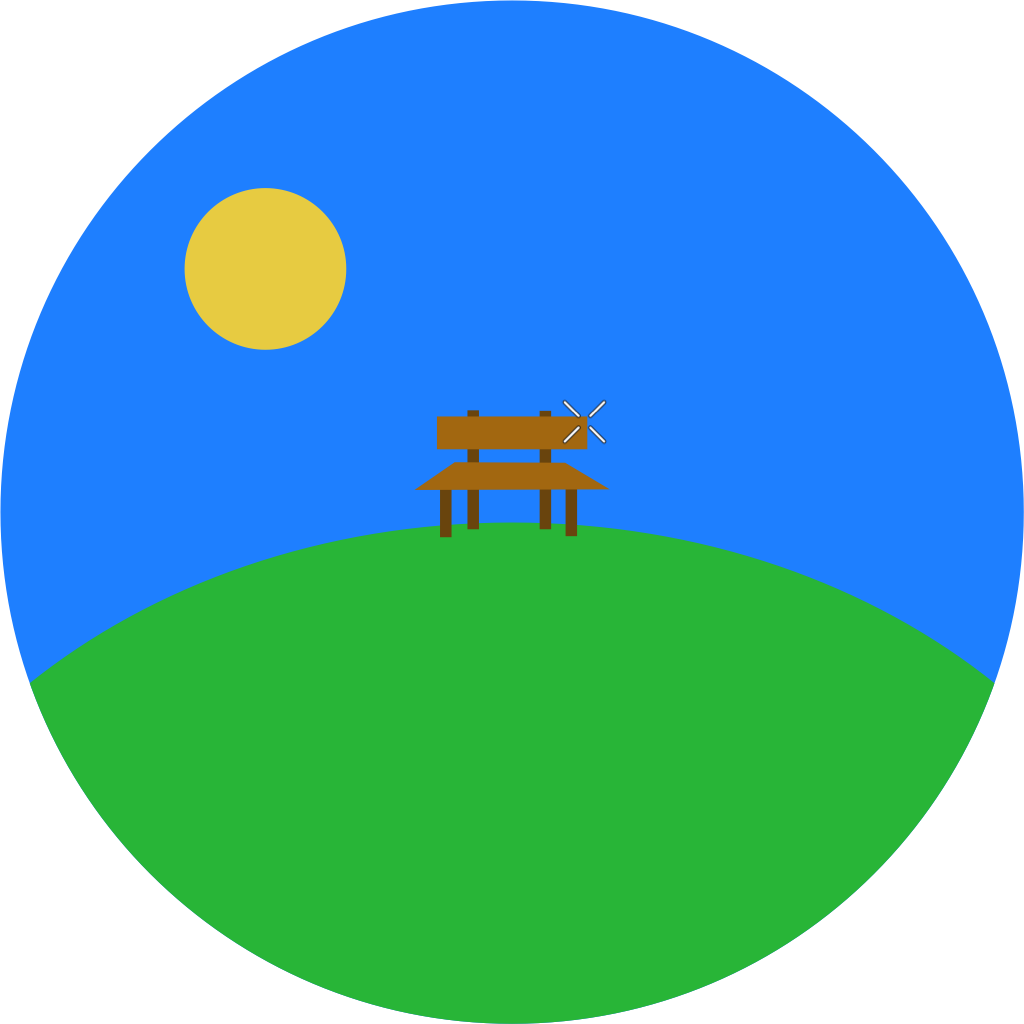
\includegraphics[scale=0.2]{parkview.png}
  \caption{A sequence diagram (if you don't look to closely)}
\end{figure}

\subsection{Configuration of plot}

\subsection{Display plots}

\subsection{Storage of benchmark results}

\subsection{Calculation of performance metrics}

\clearpage

\section{Design Data}

\subsection{Data entries}
The following data is stored in the browser's cookies:
\begin{itemize}
  \item Something
  \item Something else, probably

\begin{figure}[h!]
\subsection{Database structure}
  \centering
  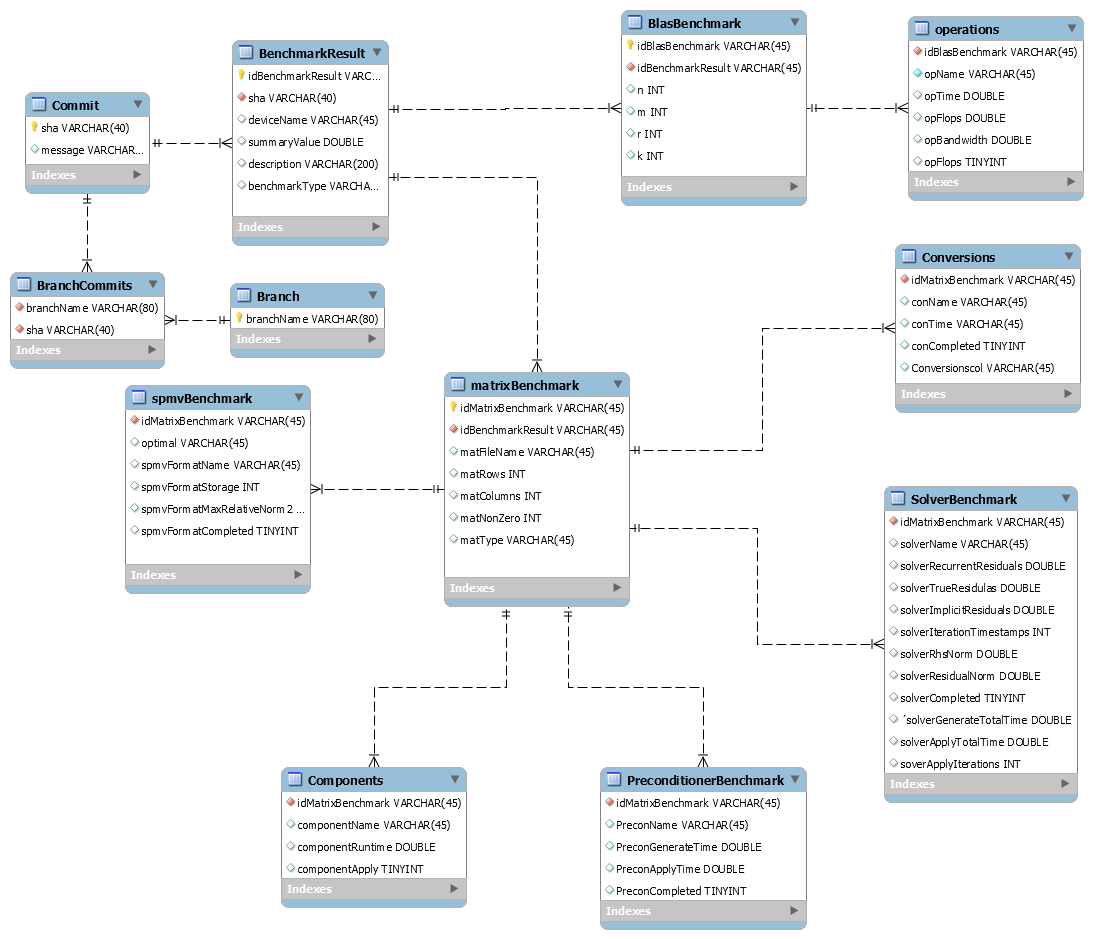
\includegraphics[scale=0.4]{ER.png}
  \caption{The database is structured according to this Entity-Relationship diagram}
\end{figure}
\end{itemize}

\clearpage


\appendix

\section{Class index}
Big list with links to all classes here, preferably in lexicographic order

\subsection{Backend}
Benchmark  \ref{b:26}\\
BenchmarkResult  \ref{b:27}\\
BenchmarkResultDatabase : BenchmarkResultStorage  \ref{b:20}\\
BenchmarkResultStorage \ref{b:1} \\
BlasBenchmarkResult : BenchmarkResult \ref{b:2} \\
BlasDatapoint \ref{b:3} \\
BlasPlotTransform  \ref{b:34}\\
BlasSinlgeScatterPlotTransform : BlasPlotTransform  \ref{b:35}\\
BlasTwoScatterPlotTransform : BlasPlotTransform  \ref{b:36}\\
BranchForBenchmark  \ref{b:28}\\
Commit  \ref{b:29}\\
Component \ref{b:4} \\
Conversion \ref{b:5} \\
ConversionBenchmarkResult : MatrixBenchmarkResult \ref{b:6} \\
ConversionDatapoint : MatrixDatapoint  \ref{b:7}\\
ConversionPlotTransform  \ref{b:37}\\
ConversionSingleScatterPlotTransform : ConversionPlotTransform  \ref{b:38}\\
ConversionTwoScatterPlotTransform : ConversionPlotTransform  \ref{b:39}\\
DataProcessor  \ref{b:40}\\
DatabaseHandler  \ref{b:21}\\
Device  \ref{b:30}\\
EmptyBenchmarkResult : BenchmarkResult  \ref{b:31}\\
Format  \ref{b:8}\\
GitApiHandler : RepositoryHandler  \ref{b:57}\\
History  \ref{b:32}\\
HistoryDatabase  \ref{b:22}\\
LazyBenchmarkResult : BenchmarkResult  \ref{b:23}\\
MatrixBenchmarkResult : BenchmarkResult  \ref{b:9}\\
MatrixDatapoint  \ref{b:10}\\
MissingBenchmarkResultException : Exception  \ref{b:25}\\
MissingCommitException : Exception  \ref{b:60}\\
Operation  \ref{b:11}\\
PlotType  \ref{b:41}\\
PostgreSQLHandler : DatabaseHandler  \ref{b:24}\\
Preconditioner  \ref{b:12}\\
PreconditionerBenchmarkResult : MatrixBenchmarkResult  \ref{b:13}\\
PreconditionerDatapoint : MatrixDatapoint  \ref{b:14}\\
PreconditionerPlotTransform  \ref{b:42}\\
PreconditionerSingleComponentBreakdownPlotTransform : PreconditionerPlotTransform  \ref{b:45}\\
PreconditionerSingleScatterPlotTransform : PreconditionerPlotTransform  \ref{b:43}\\
PreconditionerTwoScatterPlotTransform : PreconditionerPlotTransform  \ref{b:44}\\
RepositoryHandler  \ref{b:33}\\
RestHandler  \ref{b:58}\\
Solver  \ref{b:15}\\
SolverBenchmarkResult : MatrixBenchmarkResult  \ref{b:16}\\
SolverDatapoint : MatrixDatapoint  \ref{b:17}\\
SolverMultiAchievedBandwidthPlotTransform : SolverPlotTransform  \ref{b:50}\\
SolverMultiIterationCountsPlotTransform : SolverPlotTransform  \ref{b:48}\\
SolverMultiRuntimePlotTransform : SolverPlotTransform  \ref{b:47}\\
SolverMultiTimeToSolutionPlotTransform : SolverPlotTransform  \ref{b:49}\\
SolverPlotTransform  \ref{b:46}\\
SolverSingleConvergencePlotTransform : SolverPlotTransform : SolverPlotTransform  \ref{b:51}\\
SolverTwoSpeedupPlotTransform : SolverPlotTransform  \ref{b:52}\\
SpmvBenchmarkResult : MatrixBenchmarkResult  \ref{b:18}\\
SpmvDatapoint : MatrixDatapoint  \ref{b:19}\\
SpmvPlotTransform  \ref{b:53}\\
SpmvSinglePerformanceProfilePlotTransform : SpmvPlotTransform  \ref{b:54}\\
SpmvSingleScatterPlotTransform : SpmvPlotTransform  \ref{b:55}\\
SpmvTwoSpeedupPlotTransform : SpmvPlotTransform  \ref{b:56}\\
SpringRestHandler \ref{b:59}\\

\clearpage

\printnoidxglossaries

\end{document}
